\section{Framework Overview}
\label{sec:overview}

We designed a framework that analyzes, models, and detects outliers in data.
The whole system can be seen in Figure~\ref{fig:pipeline}.

\begin{figure*}
  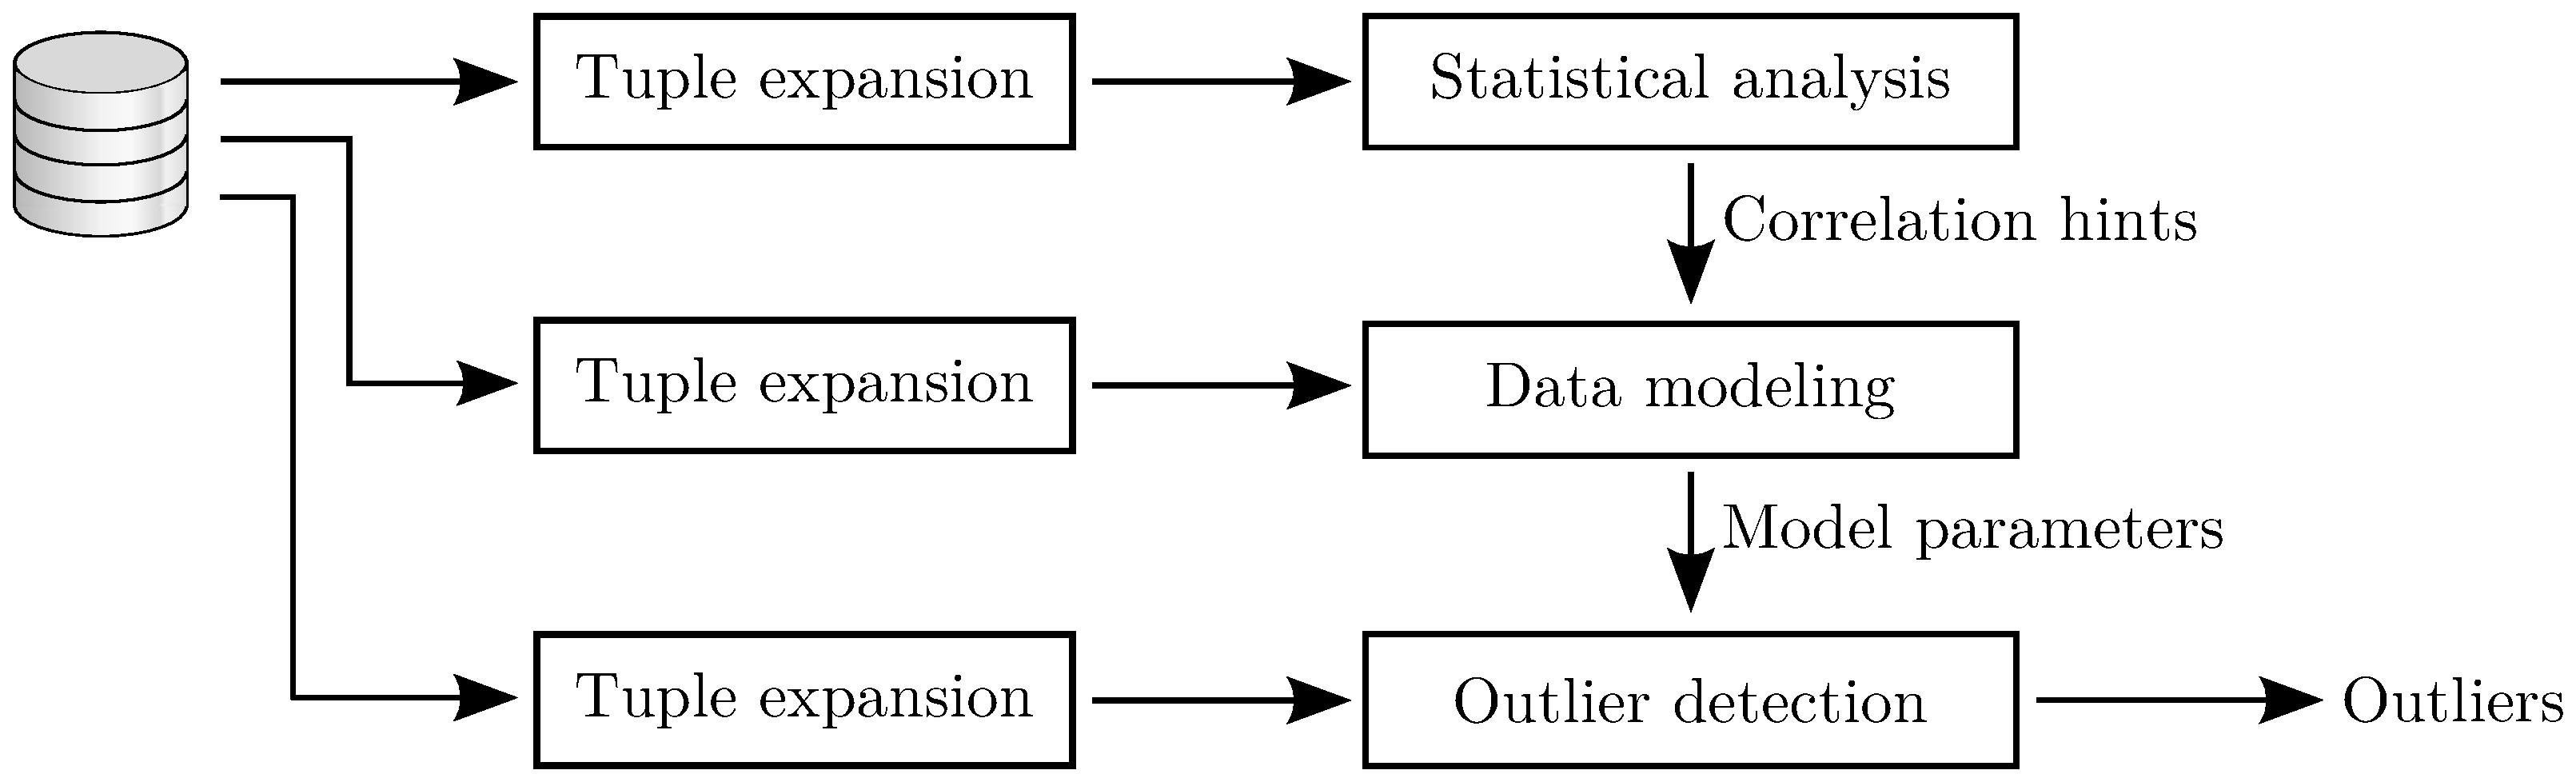
\includegraphics[width=\textwidth]{../graphics/pipeline.pdf}
  \caption{Framework pipeline}
  \label{fig:pipeline}
\end{figure*}

As a first step, tuples are read from the database and expanded: a set of type-dependent features is extracted for each field. These features express important properties of the data, such as the length of a string, or the parity of an integer.

These expanded tuples are then analyzed in order to obtain simple statistical information (mean, variance), and to detect correlations between the different fields. Next, the expanded tuples as well as the correlation information are passed to one of three data model generators, which return a model of the data.

Finally, this model is used to determine whether or not new tuples fall outside the learned data distribution. Although we mostly used the data models to detect outliers in the tuples used to learn the model parameters, the models can also be used to analyze new inputs.

From a high level view, our pipeline is implemented as a three-pass streaming algorithm, requiring no memory beyond that required to train the individual models.

The different stages of our pipeline are summarized as follows and described in detail in the following sections:

\begin{enumerate}
\item Preprocessing -- Tuples are expanded using knowledge about the database schema and field types. This process is described in detail in Section~\ref{sec:preprocessing}.
\item Statistical analysis -- The expanded data is analysed to gather basic statistics, along with correlation information. These statistics are used for modeling and outlier detection. The process is detailed in Section~\ref{sec:statistical-analysis}.
\item Data modeling -- We apply various user-selected machine-learning algorithms to build models of the data. We describe this phase in Section~\ref{sec:model-creation}
\item Outlier detection -- Using the models built in the previous stage and user-provided sensitivity thresholds, we report outliers identified by the models trained during the previous stage. This process is detailed in Section~\ref{sec:outlier-detection}.
\end{enumerate}
